
The noise, that is, unwanted deviations in the signal, can be comprised of the multiple sources which are subsequently added throughout the digital image acquisition chain. Deviations in the brightness are introduced right in the detection phase due to the discrete nature of electrons; such noise source is dubbed photon shot noise. Further fluctuations are caused during the readout of the electron charge and its subsequent amplification; for digital systems, the mapping of the voltage to discretized bit values results in the additional quantization noise. \cite{Holst2011}

\begin{figure}[h]
  \centering
  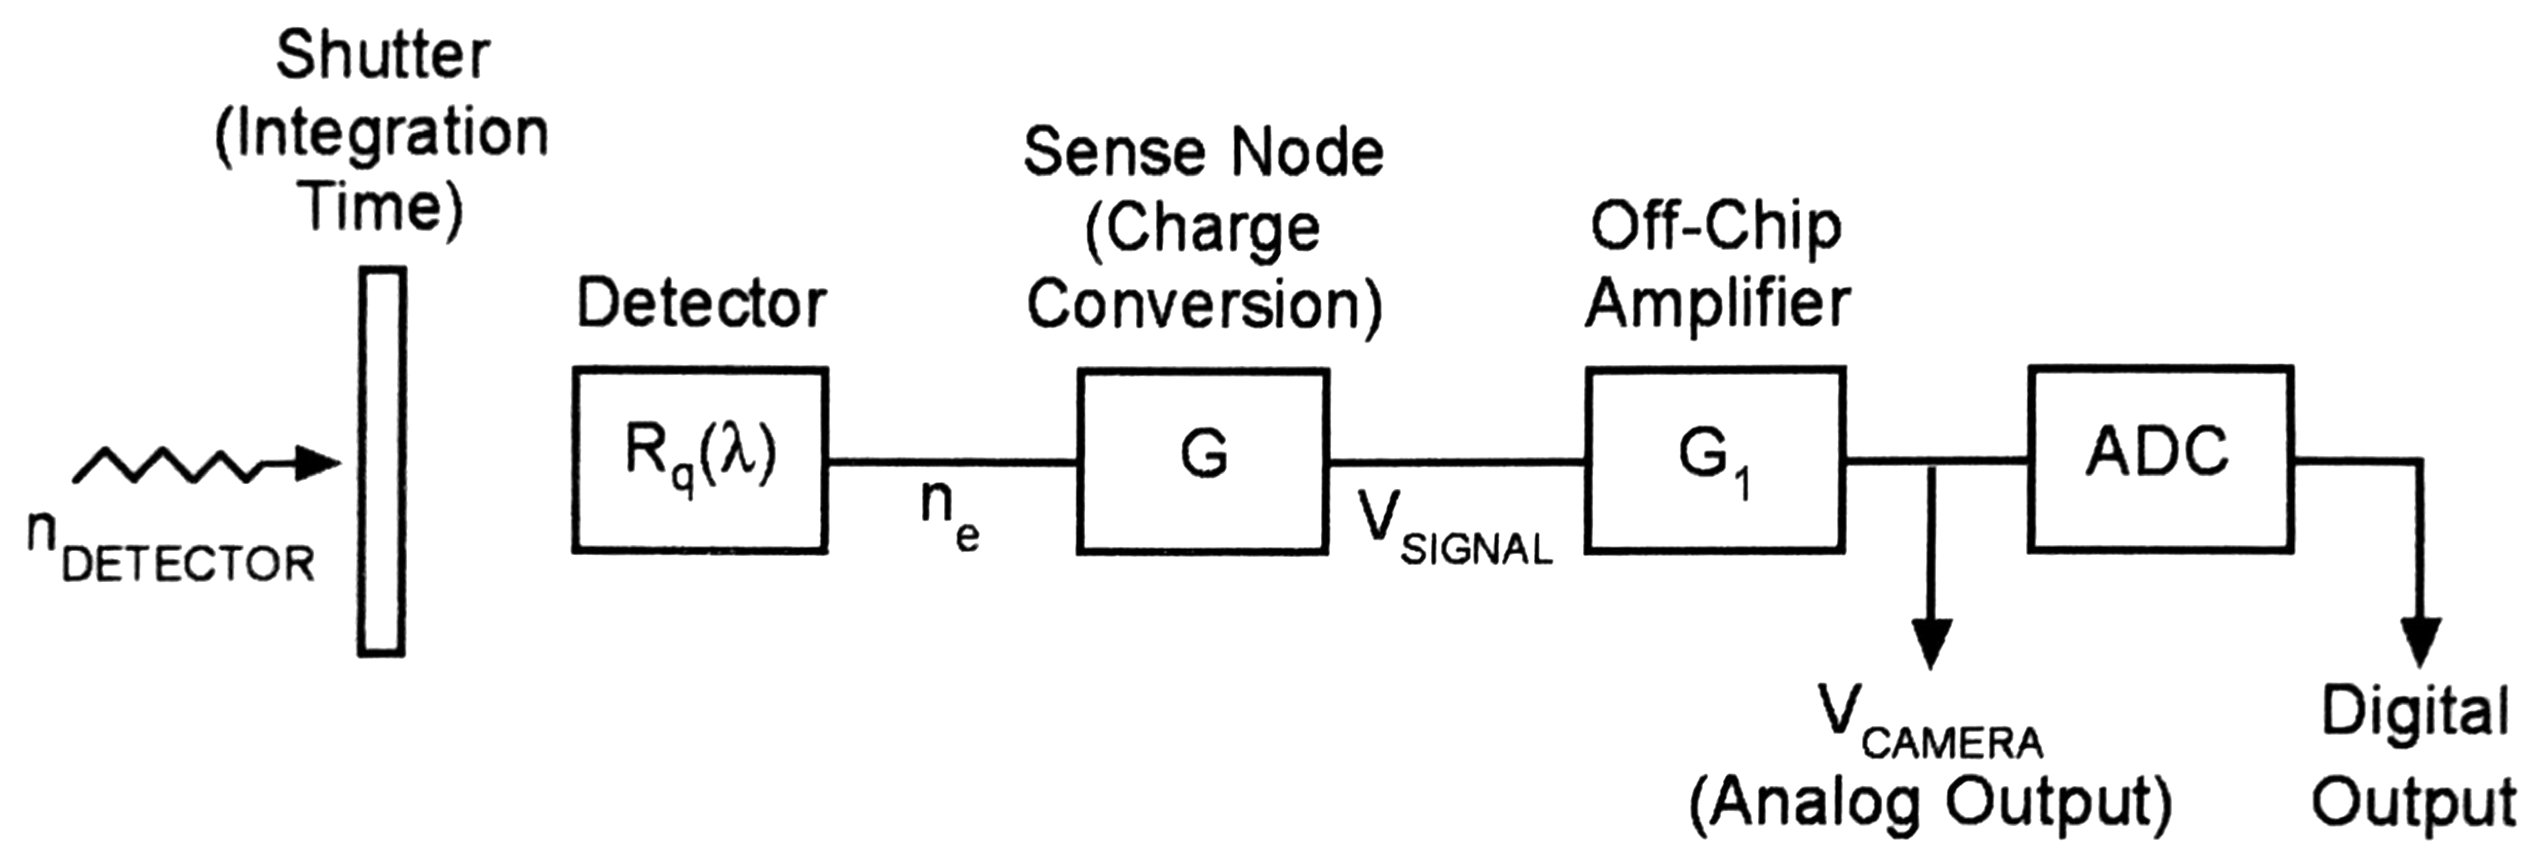
\includegraphics[width=\linewidth]{imgs/sensors/sens-signal-transfer.png}
  \caption{Signal transfer diagram in an imager, via \cite{Holst2011}. Both analog and digital outputs are considered.}
  \label{fig:sigtrans}
  \Description{Signal transfer diagram in a digital sensor. There are multiple subsystems leading to the accurate normalized representation of the signal: at first, the incident photons are detected and evaluated in their charges; this is later amplified and digitized.}
\end{figure}

\begin{figure}[h]
  \centering
  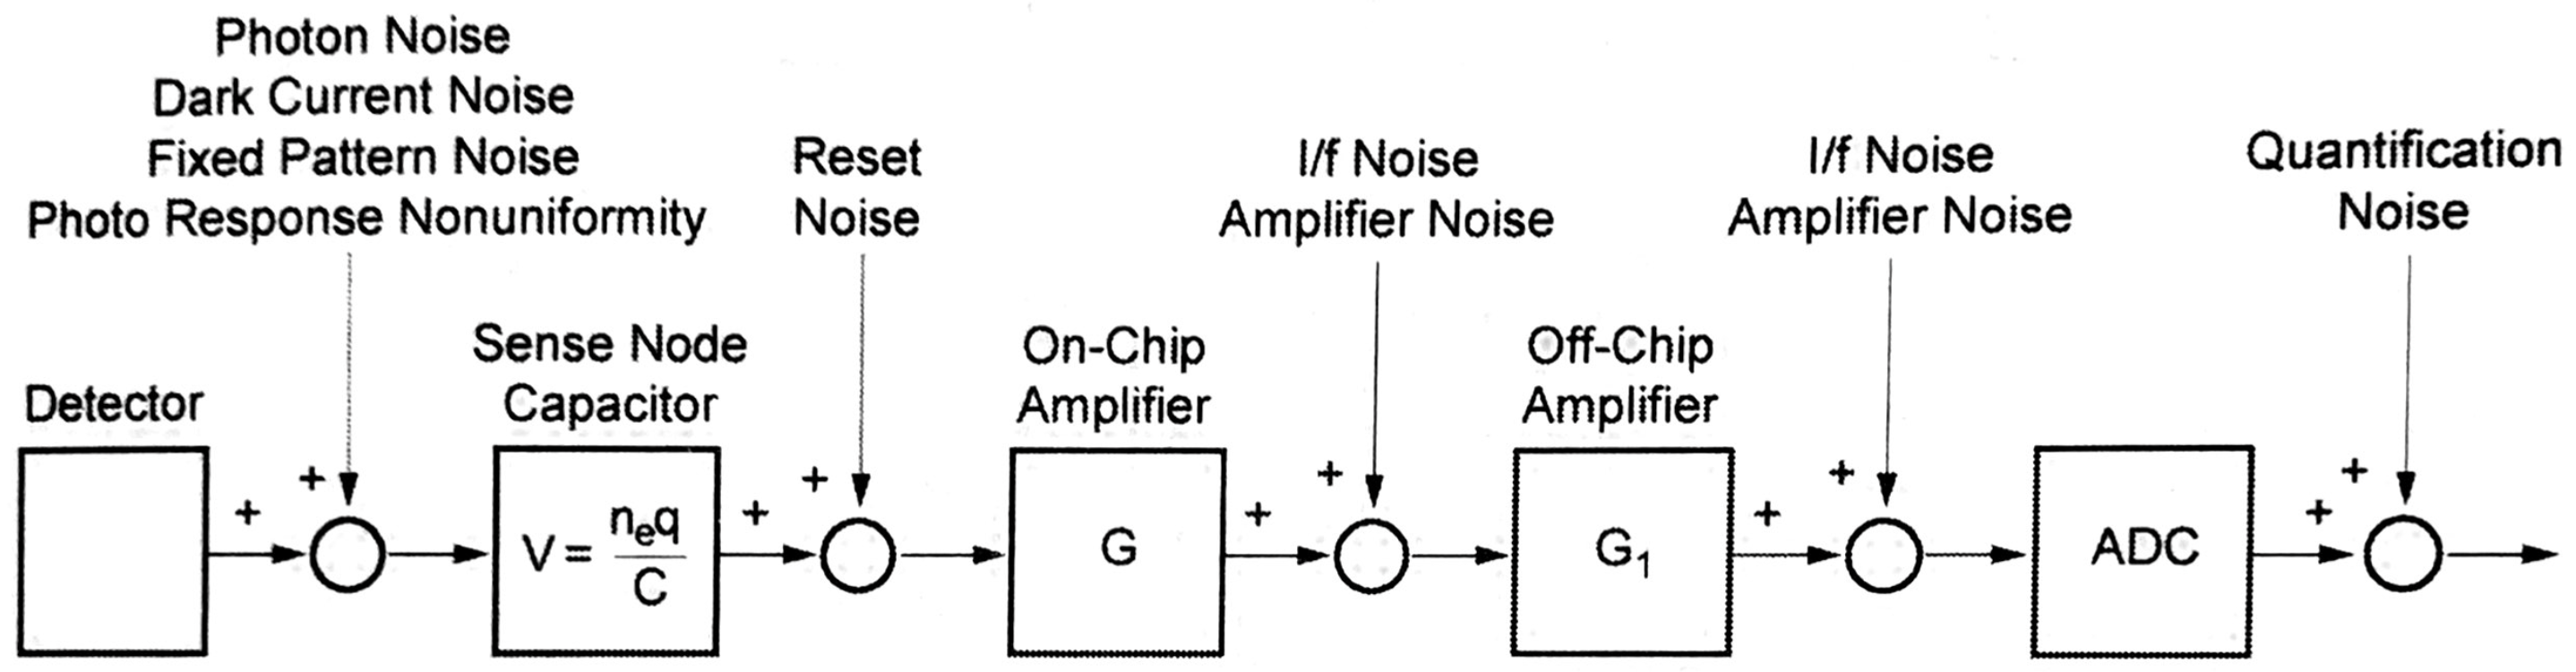
\includegraphics[width=\linewidth]{imgs/sensors/sens-noise-transfer.png}
  \caption{Noise transfer in a digital sensor, via \cite{Holst2011}. Each subsystem introduces additional noise sources which affect the subsequent signal.}
  \label{fig:noisetrans}
  \Description{For every subsystem listed in the signal transfer diagram, there is a corresponding noise source which alters the input: the photon-induced noises, reset noises, noises caused through amplifiers (off-chip and on-chip), and finally, the quanification noise.}
\end{figure}

Figures \ref{fig:sigtrans} and \ref{fig:noisetrans} show the signal transfer and the noise occuring during each step of the process, respectively. Each noise source has a different characteristics and can be attributed to either nonuniformities and physical flows of the sensor, or the natural nonstationary processes. The level of detail in the noise transfer diagram is somewhat dependent on the application, and some of the sources caused by the circuitry can be minimized through the design of the architecture, as will be shown in the further chapters. 